% ----------------------------- %
% Paper for SEXI2013            %
% http://sexi2013.org/          %
% ----------------------------- %
% Full paper:     Nov 30, 2012  %
% Notification:   Dec 17, 2012  %
% Camera-ready:   Feb  5, 2013  %
% ----------------------------- %
% Maximum pages: 2              %
% ----------------------------- %

\documentclass[runningheads,a4paper]{llncs}
\usepackage[T1]{fontenc}
\usepackage[utf8]{inputenc}


% References
\usepackage[pdftex,urlcolor=black,colorlinks=true,linkcolor=black,citecolor=black]{hyperref}
\usepackage[capitalise,nameinlink]{cleveref}
\crefname{subsection}{Subsection}{Subsections}

\usepackage{graphicx}
\usepackage{caption}
\usepackage{subcaption}

% Better typography
\usepackage[activate=compatibility]{microtype}

% Todo macro
\usepackage{color}
\newcommand{\todo}[1]{\noindent\textcolor{red}{{\bf \{TODO} #1{\bf \}}}}

% Keywords command
\newcommand{\keywords}[1]{\par\addvspace\baselineskip
\noindent\keywordname\enspace\ignorespaces#1}

\begin{document}

\mainmatter

\title{Identifying Analogue Recording Artifacts\\
In the Age of Online Video Platforms}

\titlerunning{Identifying Analogue Recording Artifacts}
\authorrunning{Thomas Steiner, Seth van Hooland, and Ruben Verborgh}

\author{Thomas Steiner\inst{1} \and
        Seth van Hooland\inst{2} \and
        Ruben Verborgh\inst{3}}

\institute{
Universitat Politècnica de Catalunya -- Department {\scshape lsi}\\
  \urldef{\emails}\path|tsteiner@lsi.upc.edu|\emails\\
\and
Université Libre de Bruxelles -- Information and Communication Science Dept.\\
     \urldef{\emails}\path|svhooland@ulb.ac.be|\emails\\
\and
Ghent University -- iMinds -- Multimedia Lab\\
  \urldef{\emails}\path|ruben.verborgh@ugent.be|\emails\\
}

\maketitle

% Ignore affiliation note numbers: start footnotes from the beginning.
\setcounter{footnote}{0}

\begin{abstract}
In this position paper, we describe how analogue recording artifacts
stemming from digitalized VHS tapes such as
grainy noises, ghosting, or synchronization problems
can be identified at Web-scale in order to
allow for filtering out content of low recording quality.
\end{abstract}

\keywords{Video Digitalization, Video Digitation, Video Home System~(VHS)}

\section{Introduction}

Online video is one of the fastest growing Internet industries.
With the latest statistics of a~well-known online video
platform\footnote{\url{http://www.youtube.com/t/press_statistics}}
of 72 uploaded hours of video per minute,
it becomes evident that efficient search, recommendation, and
navigation capabilities are required in order to use 
video platforms in a~meaningful way. 
Common online video platforms typically allow their users
(i)~to search for content based on full-text query terms
that are matched against textual descriptions
of the video like title or description,
or (ii)~to browse the archive of a~platform by category or channel,
usually based on video tags.
Users then retrieve a~top-$n$ ranked list of videos
that match a~given categorization
or query term, ranked by ranking criteria such as
\emph{relevancy}, \emph{view count},
\emph{user rating}, or \emph{upload date}.
The default ranking criteria normally being
\emph{relevancy}---a~platform-specific \emph{black box}
ranking criterium---advanced and frequently returning power-users
may prefer more transparent and traceable ranking criteria
such as the popularity-based \emph{view count}
and \emph{user rating}, or the stack-based
LIFO (last in, first out) ranking criterium \emph{upload date}.
In this position paper, we suggest a~computer vision-based
approach to a~problem with digitalized VHS content,
typically uploaded a~long time ago and thus having many views,
however, due to the oftentimes amateurish digitalization process
are of inferior quality and greatly limit the viewing experience,
albeit the poster preview may seem acceptable.
Such videos often appear prominently when users rank content
by the popularity-based ranking criterium \emph{view count}.

\section{Problem Statement}

Video denoising is the process of removing noise from a~video signal.
Typical issues with digitalized VHS videos include 
ghosting (\autoref{fig:ghosting}),
color-specific degradation,
brightness and color channel interferences,
chaotic line shift at the end of frames,
and wide horizontal noise strips (\autoref{fig:distortion}).
Such distortions can seriously limit the viewing experience
on video platforms.
In consequence, we highlight a~scalable, crowdsourced way
to identify poorly digitalized videos.

\begin{figure}
  \centering
  \begin{subfigure}[b]{0.45\linewidth}
    \centering
    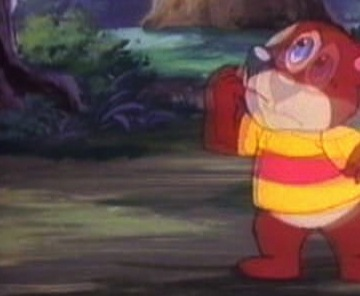
\includegraphics[width=\textwidth]{ghosting.png} 
    \caption{Ghosting
    [\url{http://goo.gl/NXJzw}]}
     \label{fig:ghosting}
  \end{subfigure}
  \begin{subfigure}[b]{0.45\linewidth}
    \centering
    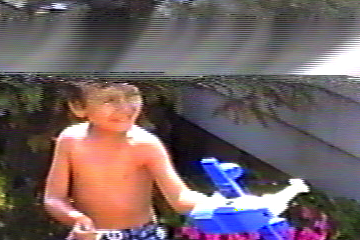
\includegraphics[width=\textwidth]{distortion.png} 
    \caption{Distortion
    [\url{http://goo.gl/zRiEQ}]}
     \label{fig:distortion}
  \end{subfigure}  
  \label{fig:artifacts}
  \caption{VHS artifacts after digitalization.}
\end{figure}

\section{Approach}
\cite{steiner2011crowdsourcing}
\cite{yang2009videonoise}
\section{Conclusion}

\bibliographystyle{splncs03}
\bibliography{references}

\end{document}
